\documentclass[10pt, letterpaper]{article}

% --- PAQUETES DE IDIOMA Y GRÁFICOS ---
\usepackage[utf8]{inputenc}
\usepackage[T1]{fontenc}
\usepackage[spanish, es-tabla]{babel}
\usepackage{graphicx}
\graphicspath{{imagenes/reporte_ejecutivo/}{imagenes/}}
\usepackage{tabularx}
\usepackage{booktabs}
\usepackage{amsmath}
\usepackage{amssymb}
\usepackage{amsfonts}
\usepackage{tikz}
\usetikzlibrary{shapes.geometric, arrows.meta, positioning}
\usepackage{float}

% --- TIPOGRAFÍA TIPO ARIAL ---
% Helvetica es la alternativa más parecida a Arial en LaTeX tradicional
\usepackage[scaled]{helvet}
\renewcommand{\familydefault}{\sfdefault}

% --- DISEÑO Y MÁRGENES ---
\usepackage[
    letterpaper,
    top=20mm,
    bottom=20mm,
    left=25mm,
    right=25mm
]{geometry}

\usepackage{fancyhdr}
\usepackage{float}
\usepackage{xcolor}
\usepackage{colortbl}
\usepackage{parskip}

% --- ESPACIADO ENTRE PÁRRAFOS E INTERLINEADO ---
% El documento pide interlineado de 5.0 pt.
% En LaTeX, esto se aproxima mejor controlando el espacio entre párrafos.
\setlength{\parskip}{5pt}
\setlength{\parindent}{0pt}

% --- COLORES PERSONALIZADOS ---
\definecolor{academicblue}{RGB}{0, 50, 100}

\usepackage[
    colorlinks=true,
    linkcolor=academicblue,
    citecolor=academicblue,
    urlcolor=academicblue
]{hyperref}

% --- ESTILO DE SECCIONES ---
\usepackage{titlesec}

\titleformat{\section}
  {\normalfont\large\bfseries\color{academicblue}}
  {\thesection}{1em}{}

\titleformat{\subsection}
  {\normalfont\normalsize\bfseries\color{academicblue}}
  {\thesubsection}{1em}{}

% Espaciado de secciones para ahorrar espacio
\titlespacing*{\section}{0pt}{10pt}{5pt}
\titlespacing*{\subsection}{0pt}{8pt}{4pt}
\titlespacing*{\paragraph}{0pt}{0pt}{5pt}

% --- ENCABEZADO Y PIE ---
\pagestyle{fancy}
\fancyhf{}
\fancyhead[L]{\small \textit{Gestor de identidades y bases de datos}}
\fancyhead[R]{\small \thepage}
\renewcommand{\headrulewidth}{0.5pt}

\begin{document}



% --- PORTADA ---
\begin{titlepage}
    \centering
    
    \vspace{1.5cm}
    
\includegraphics[width=5.5cm]{tecnologico-de-monterrey-blue} 
    
    \vspace{1cm}
    
    {\scshape\LARGE Instituto Tecnológico y de\\Estudios Superiores de Monterrey \par}
    \vspace{0.5cm}
    {\scshape\Large MA2006B.601 - Uso de álgebras modernas para seguridad y criptografía \par}
    
    \vspace{1.5cm}
    
    \hrule height 1.5pt
    \vspace{0.4cm}
    {\huge\bfseries\color{academicblue} Gestor de identidades, registros  y bases de datos \par}
    {\Large\bfseries\color{academicblue} Reporte Ejecutivo \par}

    \vspace{0.4cm}
    \hrule height 1.5pt
    
    \vspace{1.5cm}
    
    \begin{center}
    \textbf{Elaborado por:}
    \vspace{1cm}
    
    \begin{tabular}{ll}
        Álvaro Yeudiel Padilla Lobatón & A01665850 \\
        Ricardo Ballesteros Amavizca      & A01255358 \\
        Axel Gabriel Rocha Peréz      & A01067854 \\
        Ana Lidia Arteaga Bretón         & A00838732 \\
        Daniela Ortiz Blanco    & A00840140 \\
        Daniel Garnelo Martínez & A00573086
    \end{tabular}
    \end{center}
    
    \vspace{1.5cm}
    
    \begin{center}
    \large
    \textbf{Profesores:} \\
    Raúl Gómez \;|\; Alberto F. \;|\; Daniel Otero\par
    \vspace{0.2cm}
    \textbf{Fecha:} 14 de junio de 2026
    \end{center}

    \vfill
    \textbf{Casa Monarca Ayuda Humanitaria al Migrante A.B.P.} \\
    \vfill
    {\small Ingeniería en Ciencias de Datos y Matemáticas} \\
    {\small Monterrey, Nuevo León}
\end{titlepage}

% --- ÍNDICE GENERAL ---
\newpage
\tableofcontents


% --- ÍNDICE DE FIGURAS ---
\listoffigures
\newpage

\section{Resumen Ejecutivo}

El proyecto Casa Monarca consistió en el desarrollo de una aplicación web segura para la gestión de expedientes de personas atendidas por una organización de apoyo humanitario. El problema principal era la necesidad de administrar información sensible de forma ordenada, protegida y trazable, evitando accesos no autorizados, pérdida de control sobre los expedientes y exposición de datos personales.

Los objetivos iniciales fueron crear un gestor de identidades con roles definidos, proteger los datos personales mediante mecanismos criptográficos, implementar una base de datos segura y cifrada, reforzar la autenticación de usuarios críticos y registrar las acciones relevantes dentro del sistema. También se contempló la creación de cuentas de contingencia para el administrador, con el fin de mantener la continuidad operativa en caso de que la cuenta principal dejara de funcionar o no pudiera acceder al sistema.

Para lograrlo, se desarrolló una plataforma web con usuarios diferenciados por permisos, flujo de revisión de expedientes, cifrado de información sensible, certificados digitales, passkeys, bitácora de auditoría y mecanismos de protección para acciones críticas. La aplicación permite que cada usuario acceda únicamente a las funciones que corresponden a su rol, lo que ayuda a separar responsabilidades y reducir riesgos dentro del proceso.

El resultado logrado fue un sistema funcional en etapa piloto que permite crear, revisar, validar y cerrar expedientes de manera controlada. La solución mejora la seguridad del proceso al limitar el acceso según el rol del usuario, proteger los datos almacenados, reforzar la identidad de usuarios con permisos críticos y dejar evidencia de las acciones realizadas dentro del sistema.

El impacto principal del proyecto es la reducción de riesgos operativos y de seguridad en el manejo de datos sensibles. Al centralizar la información, cifrar los datos, controlar los permisos, contar con cuentas de contingencia y registrar las acciones realizadas, la aplicación fortalece la confidencialidad, integridad y trazabilidad del proceso de gestión de expedientes.

Actualmente, la aplicación cumple con las funciones principales del reto y se encuentra lista para pruebas y validación. Sin embargo, todavía existen oportunidades de mejora para futuras versiones, como preparar el sistema para un ambiente productivo, fortalecer la escalabilidad, mejorar la experiencia de usuario, robustecer la administración de llaves criptográficas y realizar pruebas con usuarios reales de Casa Monarca.


\section{Objetivos vs. Resultados}
Los objetivos iniciales del proyecto se enfocaron en desarrollar un sistema seguro para la gestión de identidades, expedientes y bases de datos dentro de Casa Monarca. La intención principal era crear una aplicación que permitiera administrar usuarios, controlar permisos, proteger información sensible, almacenar los datos de forma segura y asegurar que las acciones importantes dentro del sistema quedaran registradas para mantener trazabilidad.

Uno de los objetivos que se logró cumplir fue la implementación de un esquema de usuarios con roles diferenciados. La aplicación permite trabajar con perfiles como usuario, operativo, coordinador y administrador, cada uno con permisos específicos. Esto ayudó a separar responsabilidades y evitar que todos los usuarios tuvieran acceso completo a la información o a las funciones críticas del sistema.

Además, se incorporaron cuentas de contingencia para el administrador. Estas cuentas funcionan como una medida preventiva en caso de que, por alguna razón, la cuenta principal del administrador deje de funcionar o no pueda acceder al sistema. De esta manera, se evita que la aplicación quede bloqueada sin posibilidad de gestión, especialmente en situaciones donde sea necesario administrar usuarios, revisar configuraciones o atender acciones críticas.

También se cumplió el objetivo de proteger la base de datos y los datos sensibles de los expedientes. Para ello, se integraron mecanismos de cifrado que permiten almacenar la información de forma segura dentro de la base de datos, reduciendo el riesgo de exposición en caso de acceso indebido al archivo o a los registros almacenados. Esta parte fue fundamental porque el sistema maneja información personal y sensible, por lo que no bastaba con controlar el acceso de los usuarios, también era necesario proteger la información desde su almacenamiento.

Además, se implementaron medidas de autenticación y protección de acceso, como contraseñas protegidas, certificados digitales y passkeys, con el fin de reforzar la identidad de los usuarios con permisos críticos. Estas herramientas permiten que las acciones más importantes del sistema no dependan únicamente de una contraseña, sino de mecanismos adicionales de verificación.

Otro resultado importante fue la creación de un flujo de revisión para los expedientes. En lugar de permitir modificaciones libres, el sistema establece un proceso escalonado en el que cada expediente avanza por diferentes estados: borrador, revisión operativa, revisión de coordinación, validación y cierre. Esto permitió darle mayor orden al proceso y asegurar que cada etapa fuera atendida por el rol correspondiente.

Con respecto a los objetivos iniciales, algunas partes del proyecto se fueron adaptando durante el desarrollo. La solución final se concentró en una aplicación web funcional construida con Flask y SQLite, priorizando que el sistema pudiera ejecutarse, probarse y demostrar correctamente los mecanismos principales de seguridad. Por esta razón, se dejaron para futuras versiones mejoras relacionadas con una arquitectura más escalable, una base de datos más robusta, separación de módulos y un despliegue preparado para producción.

Dentro de los pendientes para siguientes versiones se encuentran la migración a un entorno productivo, la realización de pruebas con usuarios reales de Casa Monarca, la mejora de la interfaz de usuario y la incorporación de métricas operativas dentro del panel administrativo. También se recomienda ampliar las pruebas de seguridad, fortalecer la administración de llaves criptográficas y documentar procedimientos de respaldo, recuperación y mantenimiento del sistema.


\section{Solución Implementada}

La solución implementada consiste en una aplicación web para la gestión segura de expedientes dentro de Casa Monarca. Su función principal es permitir que la organización registre, consulte, revise y dé seguimiento a los expedientes de las personas atendidas, manteniendo la información protegida, organizada y disponible únicamente para los usuarios autorizados durante todo el proceso.

\begin{figure}[H]
    \centering
    
\includegraphics[width=0.95\textwidth]{Dashboard.png}
    \caption{Pantalla principal de la aplicación web según el rol de coordinador.}
    \label{fig:dashboard-coordinador}
\end{figure}

La Figura~\ref{fig:dashboard-coordinador} muestra la pantalla principal de la aplicación para el rol de coordinador. Desde esta vista se concentran los módulos principales del sistema, como identidades, centro de certificados, usuarios, bitácora, bandeja y creación de nuevos registros. Además, la interfaz muestra los permisos activos del usuario y el flujo de canalización de expedientes, lo que permite visualizar cómo la aplicación organiza el trabajo de acuerdo con el rol asignado.

La aplicación funciona mediante un sistema de usuarios con roles diferenciados. Cada usuario accede únicamente a las funciones que corresponden a su responsabilidad dentro del flujo de trabajo. El usuario básico puede crear expedientes, el rol operativo puede crear y consultar información, el coordinador puede revisar, consultar y actualizar expedientes, y el administrador cuenta con permisos completos para gestionar usuarios, expedientes, certificados, llaves y acciones críticas del sistema.

\begin{figure}[H]
    \centering
    
\includegraphics[width=0.85\textwidth]{CamposRegistro.png}
    \caption{Formulario de registro de beneficiarios dentro de la aplicación.}
    \label{fig:registro-beneficiario}
\end{figure}

La Figura~\ref{fig:registro-beneficiario} muestra el formulario utilizado para registrar nuevos beneficiarios dentro del sistema. Esta interfaz permite capturar de forma estructurada la información necesaria para la creación de expedientes, incluyendo datos personales y de contacto. La digitalización de este proceso contribuye a reducir errores de captura, mejorar la organización de la información y facilitar el seguimiento posterior de cada caso dentro del flujo de revisión establecido por Casa Monarca.

Como parte de la administración del sistema, también se crearon cuentas de contingencia para el administrador. Estas cuentas permiten mantener la continuidad operativa en caso de que la cuenta principal del administrador deje de funcionar, sea bloqueada o no pueda acceder al sistema. De esta forma, la aplicación no queda sin una cuenta con permisos suficientes para atender configuraciones, administrar usuarios o resolver situaciones críticas.

En términos operativos, el sistema permite que cada expediente avance por un flujo de revisión controlado. El proceso inicia con la creación del expediente en estado de borrador y posteriormente pasa por revisión operativa, revisión de coordinación, validación y cierre. Esta estructura evita que los expedientes sean modificados, validados o cerrados sin pasar por las etapas correspondientes, lo que aporta orden, control y trazabilidad al proceso.

\begin{figure}[H]
\centering
\resizebox{0.95\textwidth}{!}{
\begin{tikzpicture}[
    node distance=1.2cm,
    every node/.style={font=\small},
    etapa/.style={
        rectangle,
        rounded corners,
        draw=blue!70!black,
        thick,
        align=center,
        minimum width=3.2cm,
        minimum height=1cm,
        fill=blue!5
    },
    arrow/.style={
        -{Stealth[length=3mm]},
        thick
    }
]

\node[etapa] (borrador) {Borrador};
\node[etapa, right=of borrador] (operativa) {Revisión\\operativa};
\node[etapa, right=of operativa] (coordinacion) {Revisión de\\coordinación};
\node[etapa, right=of coordinacion] (validacion) {Validación};
\node[etapa, right=of validacion] (cierre) {Cierre};

\draw[arrow] (borrador) -- (operativa);
\draw[arrow] (operativa) -- (coordinacion);
\draw[arrow] (coordinacion) -- (validacion);
\draw[arrow] (validacion) -- (cierre);

\end{tikzpicture}
}
\caption{Flujo de revisión de expedientes dentro del sistema.}
\label{fig:flujo-expediente}
\end{figure}

La Figura~\ref{fig:flujo-expediente} muestra las etapas principales por las que pasa un expediente dentro del sistema. El proceso inicia con el registro en estado de borrador y continúa por las revisiones operativa y de coordinación, hasta llegar a la validación y cierre. Este flujo permite que cada expediente avance de forma ordenada, evitando que sea cerrado sin pasar por las revisiones correspondientes.

Además de la gestión de expedientes, la aplicación integra mecanismos de seguridad para proteger la información sensible y la base de datos. Entre ellos se encuentran el cifrado de datos almacenados, el uso de contraseñas protegidas, certificados digitales, passkeys, protección contra solicitudes no autorizadas y una bitácora de auditoría. Estos elementos permiten reducir el riesgo de exposición de información, registrar acciones relevantes dentro del sistema y reforzar la identidad de los usuarios que realizan operaciones críticas.

La base de datos fue diseñada para almacenar la información de forma segura, especialmente los datos sensibles relacionados con los expedientes. Para ello, se implementó cifrado en los campos críticos, de manera que la información no quede expuesta directamente dentro de los registros almacenados. Esto es importante porque el sistema maneja datos personales y sensibles, por lo que no solo era necesario controlar quién entra a la aplicación, sino también proteger la información desde su almacenamiento.

\begin{figure}[H]
\centering
\resizebox{\textwidth}{!}{
\begin{tikzpicture}[
    node distance=1.15cm,
    every node/.style={font=\small},
    process/.style={
        rectangle,
        rounded corners,
        draw=blue!70!black,
        thick,
        align=center,
        minimum width=5.0cm,
        minimum height=1.0cm,
        fill=blue!5
    },
    decision/.style={
        diamond,
        draw=blue!70!black,
        thick,
        align=center,
        aspect=2,
        inner sep=1.5pt,
        minimum width=4.0cm,
        minimum height=1.5cm,
        fill=blue!5
    },
    block/.style={
        rectangle,
        rounded corners,
        draw=black!70,
        thick,
        align=center,
        minimum width=4.6cm,
        minimum height=1.0cm,
        fill=gray!5
    },
    arrow/.style={
        -{Stealth[length=3mm]},
        thick
    }
]

% Nodos principales
\node[process] (login) {Inicio de sesión};

\node[process, below=of login] (cred) {Validación de credenciales};

\node[decision, below=of cred] (validas) {¿Credenciales\\válidas?};

\node[block, right=4.0cm of validas] (denegar) {Denegar acceso};

\node[process, below=of validas] (rol) {Identificar rol del usuario};

\node[process, below=of rol] (permisos) {Asignar permisos según rol};

\node[process, below=of permisos] (dashboard) {Acceso al dashboard\\correspondiente};

\node[decision, below=of dashboard] (critico) {¿Acción o módulo\\crítico?};

\node[process, left=4.4cm of critico] (funciones) {Acceso a funciones\\permitidas por su rol};

\node[process, right=4.4cm of critico] (validacion) {Validación adicional con\\passkey o certificado};

\node[decision, below=1.4cm of validacion] (correcta) {¿Validación\\correcta?};

\node[block, right=3.8cm of correcta] (bloquear) {Bloquear acción\\crítica};

\node[process, below=1.5cm of correcta, minimum height=1.1cm, text width=4.0cm] (permitir) {Permitir acción\\crítica};

\node[process, below=2.2cm of permitir, minimum width=6.5cm, minimum height=1.1cm] (proteccion) {Protección de datos y\\registro de acciones};

% Flechas principales
\draw[arrow] (login) -- (cred);
\draw[arrow] (cred) -- (validas);

\draw[arrow] (validas.east) -- node[above] {No} (denegar.west);
\draw[arrow] (validas.south) -- node[right] {Sí} (rol.north);

\draw[arrow] (rol) -- (permisos);
\draw[arrow] (permisos) -- (dashboard);
\draw[arrow] (dashboard) -- (critico);

\draw[arrow] (critico.west) -- node[above] {No} (funciones.east);
\draw[arrow] (critico.east) -- node[above] {Sí} (validacion.west);

\draw[arrow] (validacion) -- (correcta);
\draw[arrow] (correcta.east) -- node[above] {No} (bloquear.west);
\draw[arrow] (correcta.south) -- node[right] {Sí} (permitir.north);

% Convergencia final
\draw[arrow] (permitir.south) -- (proteccion.north);

\draw[arrow] (funciones.south) |- 
    ([xshift=-2.2cm]proteccion.west) -- 
    (proteccion.west);

\draw[arrow] (bloquear.south) |- 
    ([xshift=2.2cm]proteccion.east) -- 
    (proteccion.east);

\end{tikzpicture}
}
\caption{Flujo general de acceso, permisos y protección de datos.}
\label{fig:flujo-acceso}
\end{figure}

La Figura~\ref{fig:flujo-acceso} resume el flujo general de acceso, permisos y protección de datos de la aplicación. El sistema permite que los usuarios con credenciales válidas ingresen a la plataforma, pero limita las funciones disponibles de acuerdo con el rol asignado. Para acciones o módulos críticos, se solicita una validación adicional mediante passkey o certificado, fortaleciendo la seguridad sin bloquear el uso general del sistema.

\begin{figure}[H]
    \centering
    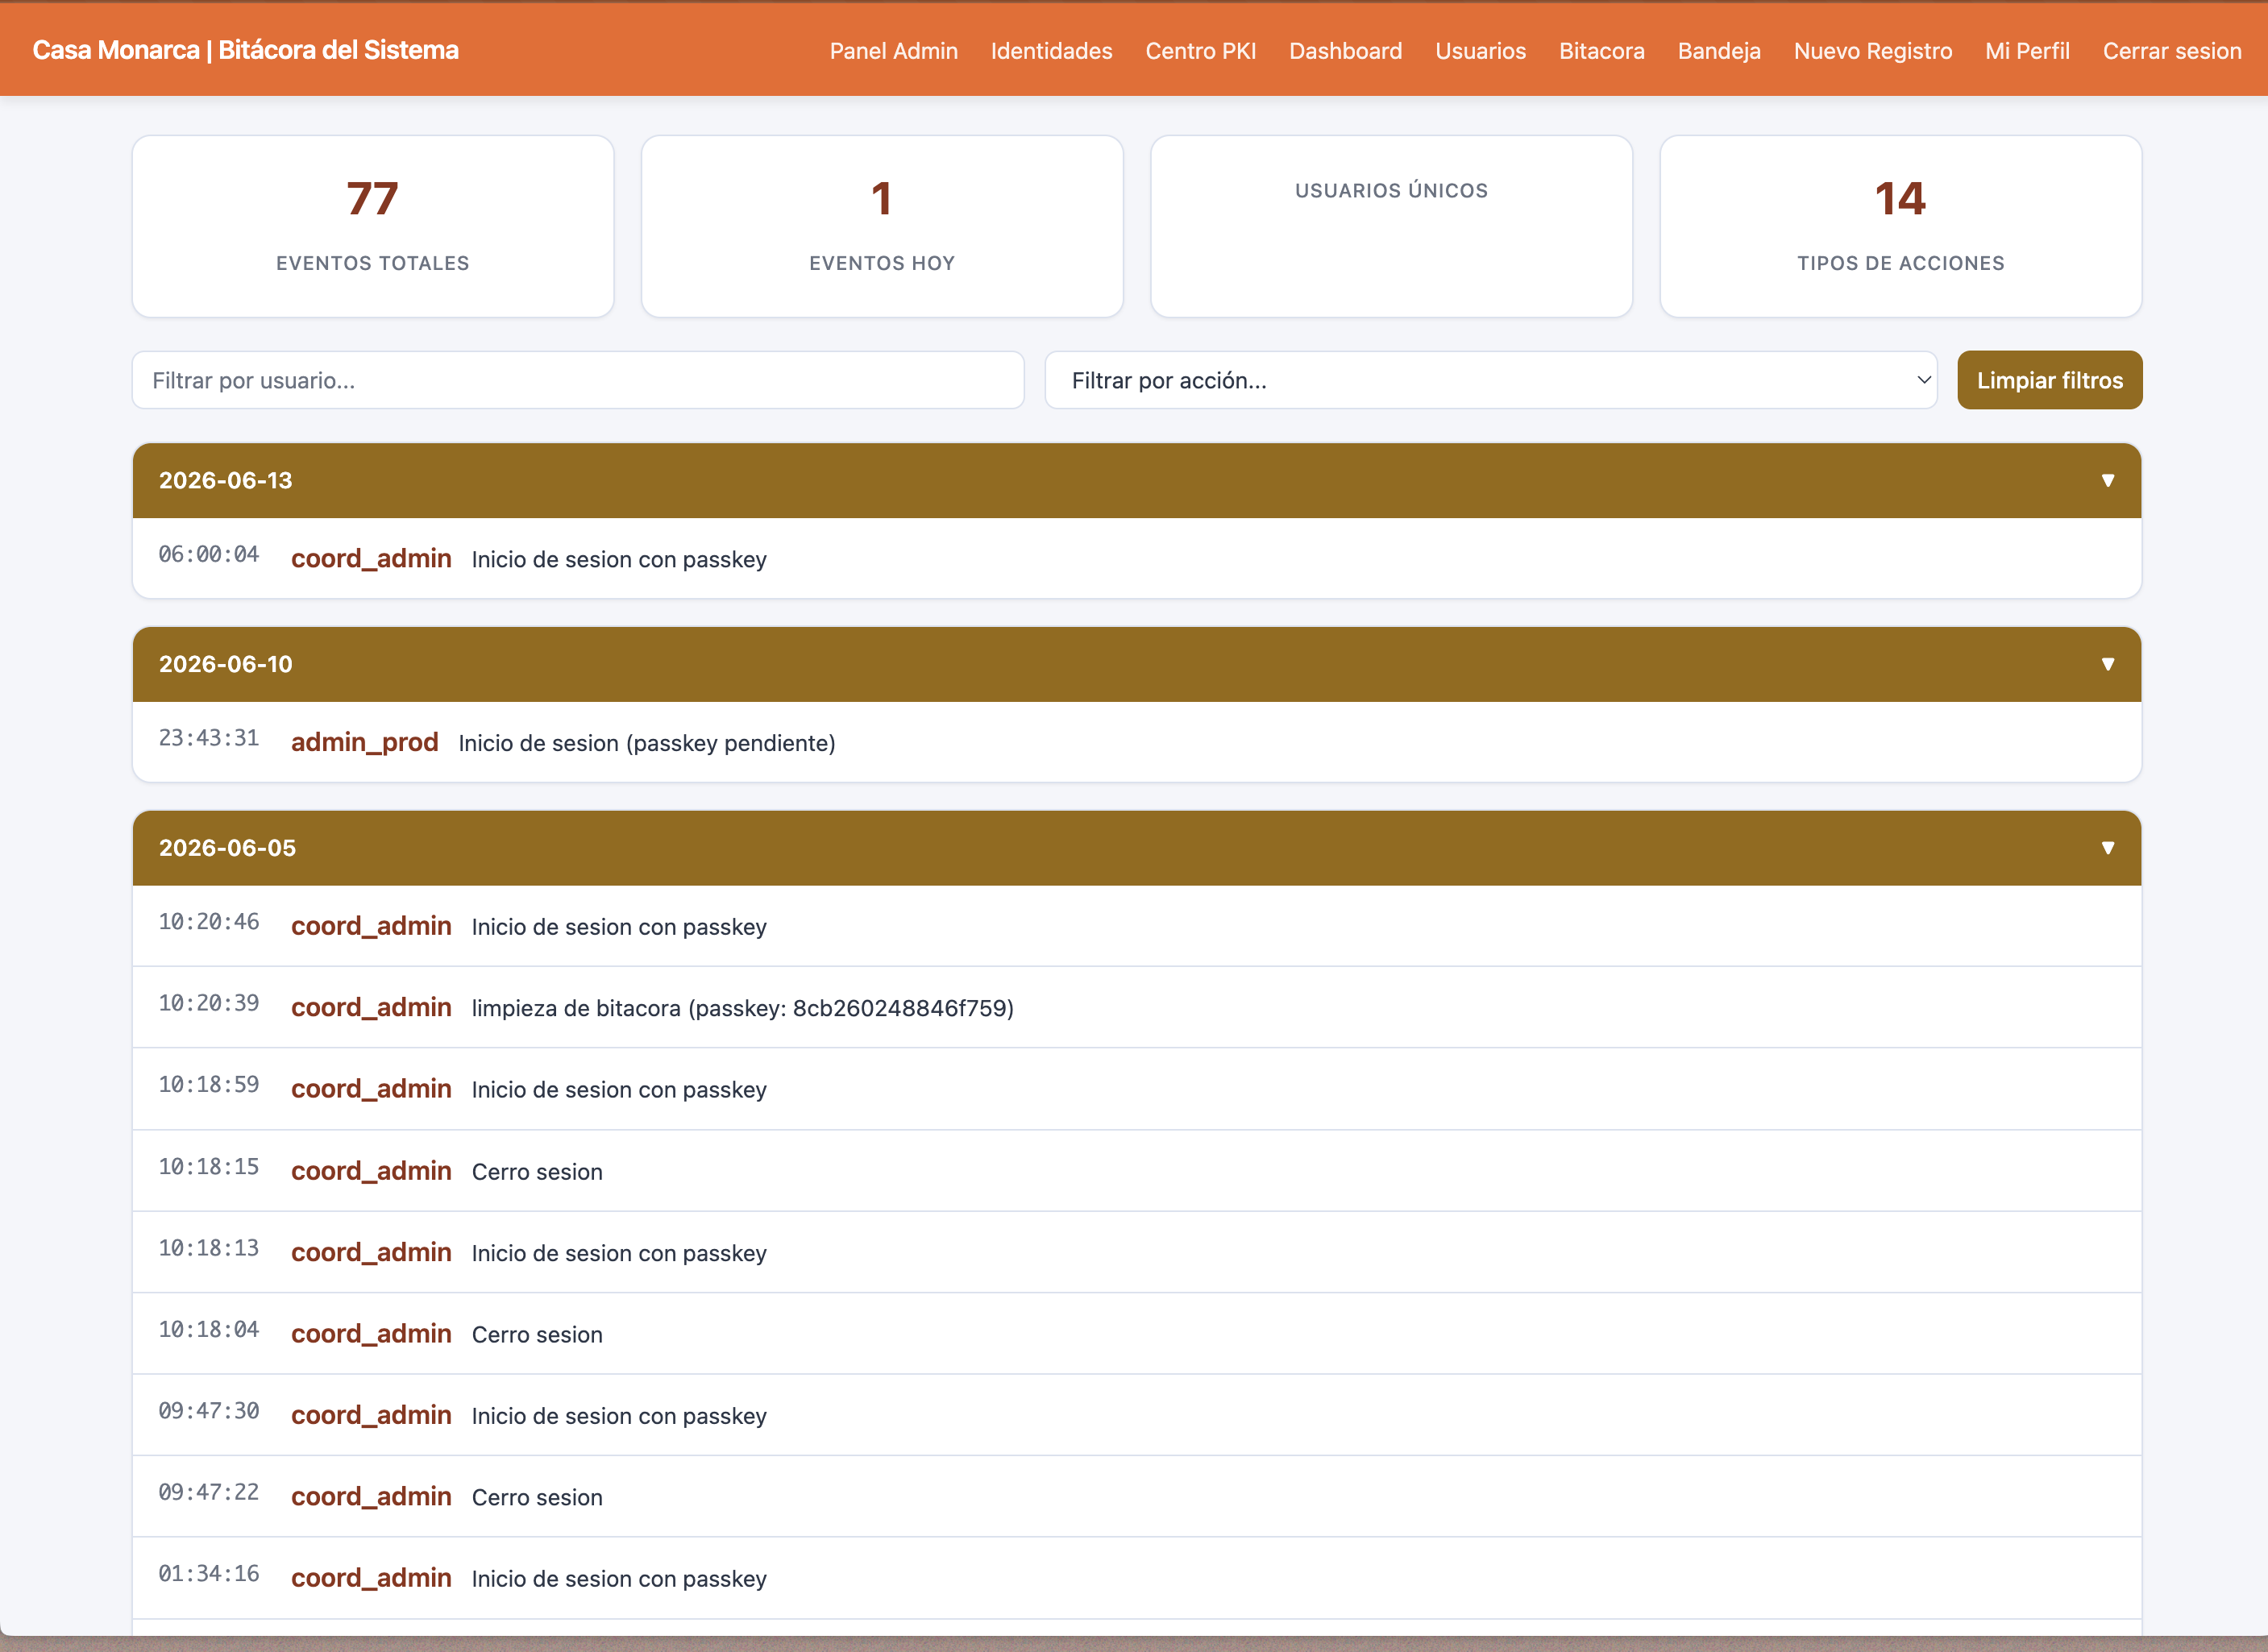
\includegraphics[width=0.95\textwidth]{Bitacora.png}
    \caption{Bitácora de auditoría de acciones realizadas en el sistema.}
    \label{fig:bitacora-sistema}
\end{figure}

La Figura~\ref{fig:bitacora-sistema} muestra la bitácora de auditoría de la aplicación, en la cual se registran eventos relevantes como inicios y cierres de sesión, así como otras acciones realizadas por los usuarios dentro del sistema. Esta funcionalidad permite mantener trazabilidad sobre el uso de la plataforma, identificar quién realizó cada operación y reforzar el control sobre acciones críticas. Además, contribuye a mejorar la supervisión del sistema y a fortalecer la protección de la información gestionada por Casa Monarca.

Los usuarios principales de la aplicación son el personal operativo, los coordinadores y los administradores de Casa Monarca. El impacto generado se refleja en una mayor seguridad en el manejo de datos personales, una mejor organización del proceso de revisión y una reducción del riesgo de accesos indebidos o modificaciones no autorizadas. También permite que la información sea más fácil de consultar y que cada acción quede asociada al usuario que la realizó.

El alcance final de la aplicación corresponde a una versión funcional en etapa piloto. Esta versión permite demostrar los componentes principales del sistema: gestión de usuarios, control de roles, creación y seguimiento de expedientes, base de datos segura, cifrado de información sensible, autenticación reforzada, cuentas de contingencia y auditoría. Sin embargo, el alcance no incluye todavía una implementación productiva a gran escala, por lo que futuras versiones deberán enfocarse en escalabilidad, pruebas con usuarios reales, mejoras de interfaz, despliegue seguro y mantenimiento operativo.


\section{Impacto de Negocio}

El impacto de negocio de la aplicación se refleja principalmente en la reducción de riesgos, la mejora en la organización del proceso y el aumento en la productividad del personal que gestiona expedientes dentro de Casa Monarca. Aunque la solución se encuentra en etapa piloto y todavía no cuenta con mediciones productivas reales, sí permite identificar beneficios claros frente a un proceso manual, disperso o poco centralizado. Además, este impacto puede sustentarse en la Ley General de Protección de Datos Personales, ya que esta ley establece bases, principios y procedimientos para garantizar el derecho a la protección de los datos personales (Cámara de Diputados del H. Congreso de la Unión, s.f.).

En términos de ahorro de tiempo, la aplicación permite concentrar la información de los expedientes en un solo sistema. Esto evita búsquedas en distintos documentos, duplicidad de registros o dependencia de archivos aislados. Al contar con un flujo definido por roles, cada usuario puede identificar con mayor claridad qué acciones le corresponden y qué expedientes requieren su revisión. Esto facilita el seguimiento de cada caso y mejora la continuidad del proceso operativo.

Respecto al ahorro económico, el beneficio se presenta de forma indirecta. Al reducir errores, accesos indebidos, pérdida de información y falta de trazabilidad, la organización disminuye la probabilidad de incidentes relacionados con el manejo inadecuado de datos sensibles. Esto puede evitar costos asociados a correcciones manuales, reprocesos, pérdida de registros, incumplimiento de políticas internas o exposición de información personal. Desde la perspectiva de la Ley General de Protección de Datos Personales, este punto es relevante porque una gestión inadecuada de los datos puede generar riesgos legales, operativos y reputacionales para la organización.

El incremento en productividad se logra porque la aplicación ordena actividades que antes podían depender de comunicación manual entre áreas. El sistema define estados para cada expediente, asigna responsabilidades según el rol del usuario y permite consultar el avance del proceso de manera más clara. De esta forma, el personal operativo, los coordinadores y los administradores pueden enfocarse en la atención y revisión de casos, en lugar de invertir tiempo adicional en organizar, buscar o validar manualmente la información.

Uno de los impactos más importantes es la reducción de errores y riesgos. La aplicación limita el acceso a la información según el rol de cada usuario, protege los datos sensibles mediante cifrado y registra las acciones relevantes en una bitácora de auditoría. Además, al contar con cuentas de contingencia para el administrador, se reduce el riesgo de que el sistema quede sin capacidad de gestión si la cuenta principal presenta algún problema. Esto fortalece la continuidad operativa y permite responder mejor ante situaciones críticas. Estas medidas también se alinean con la Ley General de Protección de Datos Personales, ya que la ley contempla la adopción de medidas de seguridad para proteger los datos personales durante su tratamiento (Cámara de Diputados del H. Congreso de la Unión, s.f.).

La implementación de una base de datos segura y con información cifrada también representa un beneficio importante para Casa Monarca. Al proteger los datos desde su almacenamiento, la aplicación reduce el riesgo de exposición en caso de accesos no autorizados al archivo o a los registros. Esto es especialmente relevante porque el sistema trabaja con información personal y sensible de las personas atendidas por la organización. En este sentido, el cifrado, el control de accesos y la trazabilidad ayudan a fortalecer el cumplimiento de los principios de seguridad y responsabilidad establecidos en la Ley General de Protección de Datos Personaless.

Para evaluar el impacto antes y después de la implementación, se proponen métricas como el tiempo promedio de creación de un expediente, el tiempo promedio de revisión por rol, el número de expedientes pendientes por etapa, el número de expedientes cerrados, la cantidad de intentos fallidos de inicio de sesión, el número de acciones críticas registradas en auditoría y la cantidad de solicitudes o modificaciones realizadas por usuario.

Antes de la aplicación, estas métricas podían ser difíciles de obtener si el proceso dependía de registros manuales o herramientas no integradas. Después de la implementación, el sistema permite generar una base para medir el avance de los expedientes, identificar cuellos de botella, supervisar acciones críticas y mejorar la toma de decisiones. Por ello, el valor principal de la solución no se limita a digitalizar expedientes, sino a crear un proceso más seguro, medible, controlado y sostenible para Casa Monarca.


\section{Lecciones y Hallazgos}

Durante el desarrollo del proyecto se identificó que uno de los aspectos que mejor funcionó fue integrar la seguridad desde el diseño de la aplicación. No se construyó únicamente un sistema para registrar expedientes, sino una solución que también considera el control de accesos, la protección de datos sensibles, la autenticación reforzada, la auditoría y la continuidad operativa. Esto permitió que la aplicación atendiera tanto la necesidad de gestionar expedientes como los riesgos relacionados con privacidad, identidad y trazabilidad.

También funcionó adecuadamente el uso de roles diferenciados dentro del sistema. La separación entre usuario, operativo, coordinador y administrador permitió organizar mejor las responsabilidades de cada perfil. De esta manera, cada persona accede únicamente a las funciones que necesita para realizar su trabajo, reduciendo el riesgo de accesos innecesarios o modificaciones no autorizadas.

Otro hallazgo importante fue la utilidad del flujo escalonado de revisión de expedientes. Al definir etapas como borrador, revisión operativa, revisión de coordinación, validación y cierre, el sistema permite representar de forma más clara cómo debe avanzar un expediente dentro de Casa Monarca. Esta estructura evita que una sola persona tenga control completo sobre todo el proceso y ayuda a que cada etapa sea revisada por el rol correspondiente.

También se observó que la combinación de diferentes mecanismos de identidad digital aporta mayor seguridad que depender únicamente de una contraseña. Las contraseñas protegidas permiten cubrir el acceso inicial al sistema, mientras que los certificados digitales y las passkeys refuerzan la autenticación de usuarios críticos. Esto ayuda a reducir riesgos como suplantación de identidad, accesos indebidos o ejecución de acciones importantes sin una verificación adicional.

Un aspecto positivo adicional fue la incorporación de cuentas de contingencia para el administrador. Este elemento permite reducir el riesgo de que el sistema quede sin capacidad de gestión si la cuenta principal del administrador deja de funcionar, se bloquea o no puede acceder por alguna razón. Con esto, la aplicación cuenta con una medida preventiva para mantener la continuidad operativa en situaciones críticas.

Dentro de los elementos que se pueden mejorar, se identificó la necesidad de preparar la aplicación para un entorno productivo más robusto. Actualmente, la solución funciona como una versión piloto, por lo que futuras versiones deberían considerar una arquitectura más modular, una base de datos más escalable, mejores herramientas de despliegue y pruebas más amplias con usuarios reales. Esto permitiría validar el desempeño del sistema en condiciones más cercanas a la operación diaria de Casa Monarca.

También se puede mejorar la experiencia de usuario. Aunque la aplicación cumple con las funciones principales, sería conveniente simplificar algunos flujos, mejorar la claridad visual de las pantallas y agregar indicadores que permitan conocer rápidamente el estado de los expedientes. Además, un panel administrativo con métricas operativas facilitaría el seguimiento de cargas de trabajo, tiempos de revisión, expedientes pendientes y acciones críticas.

Entre los riesgos detectados se encuentra la administración de llaves criptográficas. Aunque el sistema contempla cifrado para proteger la información sensible, en una implementación productiva sería necesario fortalecer los procedimientos de respaldo, recuperación, rotación y custodia de llaves. Una mala gestión de estas llaves podría provocar pérdida de acceso a información cifrada o exposición de datos sensibles.

Otro riesgo identificado es la dependencia de una arquitectura inicial concentrada en una sola aplicación. Si el sistema crece en número de usuarios, expedientes o funcionalidades, podría ser necesario separar componentes, optimizar consultas y migrar hacia una infraestructura más escalable. También se detecta el riesgo de que los usuarios no adopten correctamente mecanismos como certificados o passkeys si no reciben capacitación suficiente.

\section{Estado Actual y Próximos Pasos}

El estado actual de la aplicación corresponde a una versión piloto funcional. Esto significa que el sistema ya permite demostrar las funciones principales del proyecto, como la gestión de usuarios, el control de permisos por rol, la creación y seguimiento de expedientes, el cifrado de información sensible, el uso de certificados digitales, la autenticación mediante passkeys, las cuentas de contingencia para administrador y el registro de acciones en una bitácora de auditoría. Sin embargo, todavía no se considera una versión productiva completamente lista para operar a gran escala dentro de Casa Monarca.

La aplicación se encuentra en una etapa adecuada para pruebas, validación y retroalimentación por parte de usuarios reales. En esta fase, el objetivo principal es comprobar que los flujos implementados respondan correctamente a las necesidades operativas de la organización, especialmente en la creación, revisión, validación y cierre de expedientes. También es importante validar que los mecanismos de seguridad sean comprensibles y fáciles de usar para los distintos perfiles de usuario, ya que herramientas como certificados digitales y passkeys pueden requerir capacitación inicial.

Como siguiente paso, se recomienda fortalecer la solución para que pueda evolucionar de un piloto funcional hacia una versión productiva. Para ello, sería conveniente mejorar la infraestructura de despliegue, separar algunos componentes internos de la aplicación, ampliar las pruebas de seguridad y preparar procedimientos formales de respaldo, recuperación y mantenimiento. Estas mejoras permitirían que el sistema sea más estable, seguro y fácil de administrar en un entorno real.

En cuanto a mejoras funcionales, se recomienda optimizar la interfaz de usuario para que el personal de Casa Monarca pueda utilizar la plataforma de manera más sencilla. También sería útil agregar indicadores visuales del estado de cada expediente, filtros de búsqueda, alertas para expedientes pendientes y un panel administrativo con métricas operativas. Estas funcionalidades facilitarían el seguimiento del trabajo diario y ayudarían a identificar retrasos o cuellos de botella en el proceso.

Respecto a nuevas funcionalidades, se podrían incorporar reportes automáticos sobre expedientes creados, expedientes cerrados, tiempos promedio de revisión, actividad por usuario y acciones críticas registradas en auditoría. También se recomienda ampliar el módulo de solicitudes ARCO, mejorar la administración de certificados y passkeys, e incorporar mecanismos de notificación para avisar a los usuarios cuando un expediente requiera su revisión.

En términos de seguridad, una siguiente versión debería fortalecer la administración de llaves criptográficas, los respaldos cifrados y los procedimientos de recuperación. Aunque la aplicación ya protege información sensible mediante cifrado, en un ambiente productivo sería necesario asegurar que las llaves estén correctamente resguardadas, que existan respaldos confiables y que la organización pueda recuperar la información en caso de fallas o incidentes.

En términos de escalabilidad, una futura versión debería considerar la migración de SQLite a una base de datos más robusta, como PostgreSQL, especialmente si aumenta el número de usuarios, expedientes o consultas simultáneas. También sería recomendable modularizar el backend, separar la lógica de negocio, optimizar consultas y preparar el sistema para ejecutarse en un servidor de producción con mejores prácticas de seguridad.

\begin{thebibliography}{9}
\bibitem{lgpd}
Cámara de Diputados del H. Congreso de la Unión. (s.f.).
\textit{LEY FEDERAL DE PROTECCIÓN DE DATOS PERSONALES EN POSESIÓN DE LOS
PARTICULARES}.
Gob.mx. Recuperado el 14 de junio de 2026, de
\url{https://www.diputados.gob.mx/LeyesBiblio/pdf/LGPDPPSO.pdf}

\end{thebibliography}

\end{document}

